\documentclass[9pt,a4paper]{article}
\usepackage{amsfonts,amsmath,amsthm,amssymb}
\usepackage{graphicx,graphics,tikz,indentfirst,multirow}
\usepackage{algorithm,algorithmicx,algpseudocode,xcolor}
\usepackage[utf8x]{inputenc}
\renewcommand\figurename{Figura}
\algblockdefx{RepeatFărăWhile}{EndRepeat}{\textbf{repeat }}{}
\algnotext{EndRepeat}
\definecolor{black}{RGB}{0,0,0}

\title{\bf Laborator 7}
\author{Sîrbu Matei-Dan}
\date{26 noiembrie 2020}

\begin{document}
\maketitle

\section*{Exercițiul 1}
\subsection*{Breviar teoretic}

{\color{black}Fie $G$ un graf orientat. $G$ este un \textit{arbore cu rădăcina r}, dacă există $G$ un vârf $r$ din care oricare alt vârf poate fi ajuns printr-un drum unic.

Definiția este valabilă și pentru cazul unui graf neorientat, alegerea unei rădăcini fiind însă în acest caz arbitrară: orice arbore este un arbore cu rădăcină, iar rădăcina poate fi fixată în oricare vârf al său. Aceasta, deoarece dintr-un vârf oarecare se poate ajunge în orice alt vârf printr-un drum unic.

\begin{figure}[htbp]
    \centering
    \begin{minipage}[t!]{0.3\textwidth}
        \begin{tabular}{cc}
            nivelul & adâncimea \\
                    &           \\
            2       & 0         \\
                    &           \\
                    &           \\
                    &           \\
            1       & 1         \\
                    &           \\
                    &           \\
                    &           \\
                    &           \\
            0       & 2         \\
                    &           \\
                    &           \\
        \end{tabular}
    \end{minipage}
    \begin{minipage}[t!]{0.65\textwidth}
        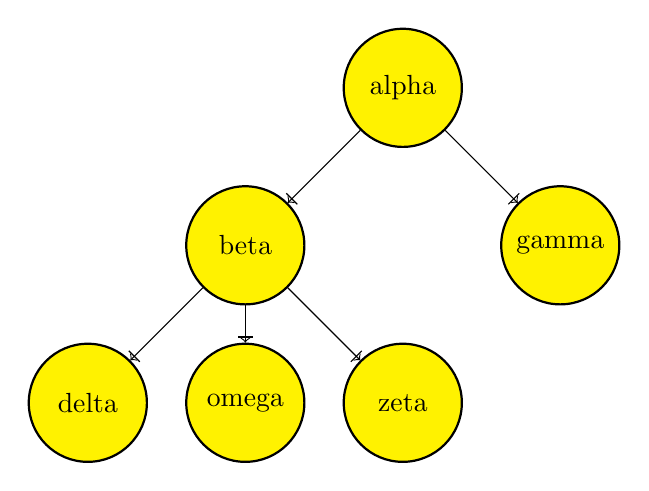
\begin{tikzpicture}[every node/.style={draw=black,thick,circle,inner sep=0pt,fill=yellow}]
            \node[minimum size=1.5cm] (A) at (0,0) {alpha};
            \node[minimum size=1.5cm] (B) at (-2,-2) {beta};
            \node[minimum size=1.5cm] (G) at (2,-2) {gamma};
            \node[minimum size=1.5cm] (D) at (-4,-4) {delta};
            \node[minimum size=1.5cm] (O) at (-2,-4) {omega};
            \node[minimum size=1.5cm] (Z) at (0,-4) {zeta};

            \path [-|>] (A) edge (B);
            \path [-|>] (A) edge (G);
            \path [-|>] (B) edge (D);
            \path [-|>] (B) edge (O);
            \path [-|>] (B) edge (Z);
        \end{tikzpicture}
    \end{minipage}
    \caption{Un arbore cu rădăcină.}
    \label{fig:arbore}
\end{figure}

Când nu va fi pericol de confuzie, vom folosi termenul ,,arbore'', în loc de termenul corect ,,arbore cu rădăcină''. Cel mai intuitiv este să reprezentăm un arbore cu rădăcină, ca pe un arbore propriu-zis. În figura \ref{fig:arbore}, vom spune că \textit{beta} este \textit{tatăl} lui \textit{delta} și fiul lui
\textit{alpha}, că \textit{beta} și \textit{gamma} sunt \textit{frați}, că \textit{delta} este un \textit{descendent} al lui \textit{alpha}, iar \textit{alpha} este un \textit{ascendent} al lui \textit{delta}.}

\newpage
\section*{Exercițiul 2}

Presupunem, pentru simplificare, că vârfurile sunt numerotate, $V = \{1, 2, ..., n\}$, vârful 1 fiind sursa, și că matricea $L$ dă lungimea fiecărei muchii, cu $L[i,j] = +\infty$, dacă muchia ($i,j$) nu există. Soluția se va construi în tabloul $D[2 .. n]$. Algoritmul este:

\begin{algorithm}
    \begin{algorithmic}
        \Procedure{Dijkstra}{$L[1 .. n, 1 .. n]$} \Comment{inițializare}
        \State{$C \gets \{2, 3, \dots, n\}$} \Comment{S = V \textbackslash C există doar implicit}
        \For{$i \gets 2$ \textbf{to} {$n$}}
        \State{$D[i] \gets L[1, i]$} \Comment{bucla Greedy}
        \EndFor
        \RepeatFărăWhile{$n-2$ \textbf{times}}
        \State{$v \gets \text{vârful din }C \text{ care minimizează } D[v]$}
        \State{$C \gets C \backslash \{v\}$} \Comment{și, implicit, $S \gets S \cup \{ v\}$}
        \For{fiecare $w \in C$}
        \State{$D[w] \gets \text{min}(D[w], D[v] + L[v, w])$}
        \EndFor
        \EndRepeat
        \State{\Return{$D$}}
        \EndProcedure
    \end{algorithmic}
\end{algorithm}

Pentru graful din Figura \ref{fig:graf}, pașii algoritmului sunt prezentați în Tabelul \ref{tbl:algoritm}.

Observăm că $D$ nu se schimbă dacă mai efectuăm o iterație pentru a-l scoate și pe \{2\} din $C$. De aceea, bucla greedy se repetă de doar $n-2$ ori.

Se poate demonstra următoarea proprietate:

\begin{figure}[htbp]
    \centering
    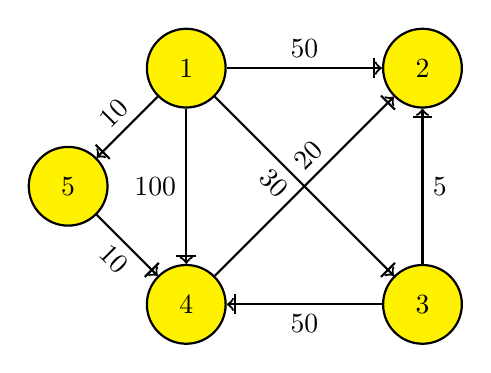
\begin{tikzpicture}[fatnode/.style={draw=black,thick,circle,inner sep=0pt,fill=yellow,minimum size=1cm}]
        \node[fatnode] (1) at (0,0) {1};
        \node[fatnode] (2) at (3,0) {2};
        \node[fatnode] (3) at (3,-3) {3};
        \node[fatnode] (4) at (0,-3) {4};
        \node[fatnode] (5) at (-1.5,-1.5) {5};

        \draw [thick, -|>] (1) -- (2) node[midway, above] {50};
        \draw [thick, -|>] (1) -- (4) node[midway, left] {100};
        \draw [thick, -|>] (1) -- (5) node[midway, sloped, above] {10};
        \draw [thick, -|>] (5) -- (4) node[midway, sloped, below] {10};
        \draw [thick, -|>] (3) -- (4) node[midway, below] {50};
        \draw [thick, -|>] (3) -- (2) node[midway, right] {5};
        \draw [thick, -|>] (1) -- (3) node[midway, sloped, below left] {30};
        \draw [thick, -|>] (4) -- (2) node[midway, sloped, above right] {20};
    \end{tikzpicture}
    \caption{Un graf orientat.}
    \label{fig:graf}
\end{figure}

\begin{figure}[htbp]
    \renewcommand\figurename{Tabelul}
    \setcounter{figure}{0}
    \centering
    \begin{tabular}{ccll}
        \textbf{Pasul} & $v$ & $C$            & $D$               \\
        inițializare   & --- & \{2, 3, 4, 5\} & [50, 30, 100, 10] \\
        1              & 5   & \{2, 3, 4\}    & [50, 30, 20, 10]  \\
        2              & 4   & \{2, 3\}       & [40, 30, 20, 10]  \\
        3              & 3   & \{2\}          & [35, 30, 20, 10]
    \end{tabular}
    \caption{Algoritmul lui Dijkstra aplicat grafului din Figura \ref{fig:graf}.}
    \label{tbl:algoritm}
\end{figure}

\end{document}